\documentclass[12pt]{article}
\usepackage{esqu1}
\pagestyle{fancy}

\lhead{Brandon Lin}
\chead{Differential Equations}
\rhead{Spring 2016}

\begin{document}


\title{Differential Equations}
\author{Brandon Lin\\Stuyvesant High School\\Spring 2016\\Teacher: Mr. Stern}
\maketitle
\newpage

\tableofcontents 

\newpage
\section*{Introduction}

\begin{itemize}
\item Email: jstern@stuy.edu
\item Office: Room 351, periods 5,7,9
\end{itemize}

\section{2/3/16: Background on $\mathbb{R}$; Basic Existence Question of ODE's}
\subsection{Romeo and Juliet}
\[
\begin{cases}
R' = aR + bJ \\
J' = cR + dJ 
\end{cases}
\]

These equations model the rate of change of Romeo's and Juliet's feelings. We call this a \textbf{linear system of two coupled differential equations of first order in two unknowns}. 
\begin{itemize}
\item What makes it linear is that the functions and variables appear in a linear fashion. 
\item What makes it coupled is that both equations have both $R$ and $J$ in them.
\item An \textbf{uncoupled system} would look like:
\[
\begin{cases}
R' = aR \\
J' = bJ
\end{cases}
\] 
\item First-order refers to the fact that all the derivatives are the first derivatives.
\end{itemize}
``Identically cautious lovers'':
\[
\begin{aligned} 
R' = aR + bJ &\quad a<0, b>0 \\
J' = bR + aJ &\quad |a| > |b|
\end{aligned}
\]

We may have initial conditions, $R(0)$ and $J(0)$, and plot them on a \textbf{phase plane} with $R$ against $J$. In this case, no matter where the starting point is, the trajectory will go towards a \textbf{stable node}.
\begin{figure}[h!]
\centering
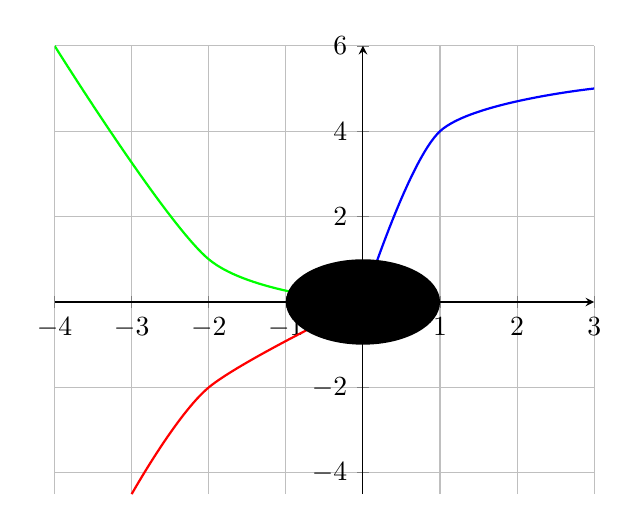
\begin{tikzpicture}
\begin{axis}[grid=major,axis x line=middle,
             axis y line=middle,
             after end axis/.code={
  }]

\addplot[color = green, smooth, thick,] coordinates
    {(-4,6) (-2,1) (0,0)};
\addplot[color = blue, smooth, thick] coordinates
    {(3,5) (1,4) (0,0)};
\addplot[color = red, smooth, thick] coordinates
    {(-3,-4.5) (-2,-2) (0,0)};
\fill[black] (axis cs:0,0) circle (1);
\end{axis}
\end{tikzpicture}
\end{figure}

In the case of $|a| < |b|$, points will move asymptotically towards $R = -J$ and $R = J$. \\
In the case of $|a| = |b|$, points will cycle around the origin infinitely.
\newpage

\subsection{Supremum and Infimum of a Set $\mathcal{A} \subseteq \mathbb{R}$}
\begin{itemize}
\item If $\mathcal{A} \in (-\infty, b]$ for some $b \in \mathbb{R}$, we say $\mathcal{A}$ is bounded above, and that $b$ is an \textbf{upper bound} for $A$. 
\end{itemize}

\begin{theorem}[Supremum Theorem]
If $\mathcal{A} \in \mathbb{R}$, $A \neq \emptyset$, and $A \subseteq (-\infty, b]$ for some $b \in \mathbb{R}$, then there exists $a \in \mathbb{R}$ such that $\mathcal{A} \subseteq (-\infty, a ]$ but if $x < a$, then $\mathcal{A} \not \subseteq (-\infty, x]$. \\
We write $a = \sup{\mathcal{A}}$, call it the \textbf{supremum} of $\mathcal{A}$.
\end{theorem}

Why is this necessary? Consider the set $\mathcal{A} = \{-\frac{1}{n} | n \in \mathbb{N} \}$. It does not have a maximum persay, but it has a supremum $\sup{\mathcal{A}} = 0$. \\ \\
Consider this example: What is $\sup{(-\mathbb{N})}$? It is -1, which also happens to be the maximum of the set.
e
\begin{theorem}
If max $\mathcal{A}$ exists as a real number, then $\sup{\mathcal{A}} = \max{\mathcal{A}}$.
\end{theorem}

But to answer all these questions, we need to figure out: what exactly are the real numbers? 

\subsection{What is $\mathbb{R}$?}
Let $x = (s,N,d_1,d_2,d_3,\dots,d_k,\dots)$, where:
\begin{itemize}
\item $s \in \{+1,-1\}$
\item $N \in \mathbb{Z}$
\item $d_k \in \mathbb{D} = \{0,1,2,3,4,5,6,7,8,9\}$
\item $\neg (\exists k : d_{k+1} = d_{k+2} = \dots = 0)$, this is to prevent multiple sequences from being the same number
\end{itemize}

In this case, ``2.49'' is shorthand for $(+1,2,4,8,9,9,9,\dots)$

\section{2/4/16: Background in $\mathbb{R}$; Fundamental Existence/Uniqueness Question}

\subsection{Supremums and Infimums in Integrals}
\begin{theorem}[Supremum/Infimum Theorem] 
\
\begin{enumerate}
\item If $\mathcal{A}$ is a non-empty set of $\mathbb{R}$, and is bounded above (i.e. $\mathcal{A} \subseteq (-\infty, b]$ for some $b \in \mathbb{R}$), then there is a \underline{least} upper bound for $\mathcal{A}$, namely $a \in \mathbb{R}$ such that
\begin{enumerate}
\item $\mathcal{A} \subseteq (-\infty, a]$
\item if $x < a$, then $\mathcal{A} \not \subseteq (-\infty, x]$
\end{enumerate}
This $a$ is called the called the \textbf{supremum} of $\mathcal{A}$, written $\sup{A}$.
\item $\inf{A}$. This is the \underline{greatest lower bound} for $\mathcal{A}$, or the \textbf{infimum}, provided $\mathcal{A} \neq \emptyset$ and $\mathcal{A}$ has a lower bound at all.
\end{enumerate}
\end{theorem}

Recall that the Riemann integral is taking the limit of a partition over an interval $[a,b]$. But when we take the limit, we make the mesh of the partition, $\norm{\mathcal{P}}$, approach zero, where \[ \mathcal{P} = \max_{1 \le i \le n}{\Delta x_i} \]

To fix this, we can define: \[ \lowint_a^b f(x) \ dx = \sup\left\{ \sum_{i=1}^n[\inf\{f(x) \ | \ x_{i-1} \le x \le x_i \}\Delta x_i] \ \middle| \ a = x_0 < x_1 < \dots < x_n = b\right\} \] 

This is a ``down-and-up'' procedure. The sum of the rectangle areas is a down approximation since we use the minimum possible height to find the area. Then, we take the supremum of that, since for any lower approximation there will always be a higher approximation. Turns out there will never be a maximum; that's why we take the supremum. This is a \textbf{lower Riemann sum}.

We can also define the same thing for an \textbf{upper Riemann sum}: \[ \upint_a^b f(x) \ dx = \inf\left\{ \sum_{i=1}^n[\sup\{f(x) \ | \ x_{i-1} \le x \le x_i \}\Delta x_i] \ \middle| \ a = x_0 < x_1 < \dots < x_n = b\right\} \]

Therefore, the following inequality is true: \[ \lowint_a^b f \le \upint_a^b f \]

If these two are equal, then we say that $f$ is \textbf{Riemann integrable}. \\ \\

Here's an example of a function that is NOT Riemann integrable:
\[ f(x) = 
\begin{cases}
0 \text{ if } x \in \mathbb{Q} \cap [0,1] \\
1 \text{ if } x \in [0,1]\backslash \mathbb{Q}
\end{cases}
\]

Note that $\lowint_0^1 f = 0$ and $\upint_0^1 f = 1$, so this is not Riemann integrable.

\subsection{Real Numbers, Again}
We have shorthand for our previous definition of the real numbers.
\[ \mathbb{R} = \{0\} \cup \{(s,N,d_1,d_2,\dots, d_k,\dots \ | \ s \in \{-1,+1\}, N \in \mathbb{Z}^+, d_k \in \mathbb{D}, \text{no 0-tail} \}\]
and the positive reals: \[ \mathbb{R}^+ = \{(s,N,d_1,d_2,\dots) \ | \ s = +1\} \]
Let us write  $x = \underline{N}.\underline{d_1d_2d_3\dots}$ and $y = \underline{M}.\underline{e_1e_2e_3\dots}$. \\ \\
We also define negation as: \[ -(s,N,d_1,d_2,\dots) \coloneqq (-s,N,d_1,d_2,\dots) \]
Then we can define the ``less than'' operation as follows:
\begin{itemize}
\item If $x,y \in \mathbb{R}^+$, then $x<y$ if either $N < M$ or $N =M$ and $d_1 < e_1$ or $N = M$, $d_1 = e_1$ and $d_2 < e_2$, or...
\item $0<x$ if $x \in \mathbb{R}^+$
\item $x < 0$ if $x \in \mathbb{R}^+$
\item  $x<y$ if $x \in \mathbb{R}^-, y \in \mathbb{R}^+$. 
\item $x,y \in \mathbb{R}^-$, and $x<y$ if $-y < -x$
\end{itemize}

\section{2/5/16: Fundamental Existence of Uniqueness Theorem}

\subsection{Terminology}
A \textbf{differential equation} is a relation between one or more unknown functions and at least some (but finitely many) of their derivatives, plus the independent variables. \\ \\ Examples: 
\[ 
\begin{aligned}
y' + 2xy - x^2 &= 3 \\ 
y''' + 2x^2y'' - 3x^3y' +xy - x^5 + 1 &= 0 \\
(y')^{y''} - e^{y'''} + x &= 0 \\
\end{aligned}
\]
Or,

\[ 
\pvec{y}' = {\bf A}(x)\vec{y} 
\]
where 
\[
\pvec{y} = \vec{y}(x) = 
\begin{bmatrix}
y_1(x) \\
y_2(x) \\
\vdots \\
y_n(x)
\end{bmatrix}
\]

\[
{\bf A}(x) = 
\begin{bmatrix}
a_{11}(x) & a_{12}(x) & \cdots & a_{1n}(x) \\
a_{21}(x) & a_{22}(x) & \cdots & a_{2n}(x) \\
\vdots & \vdots & \ddots & \vdots \\ 
a_{n1}(x) & a_{n2}(x) & \cdots & a_{nn}(x) 
\end{bmatrix}
\]

\subsection{A Treatise on PDE's}
There are two different types of differential equations: ODE's (ordinary, where all unknown functions depend on a single, same independent variable) and PDE's (partial, anything else). 

\[ \text{Wave equation: } \frac{\partial^2u}{\partial x^2} = c^2 \frac{\partial^2u}{\partial t^2} \]
\[ u = g(x-t) + h(x+t) \]

\section{2/9/16: Basic Existence and Uniqueness Theorem}

\begin{theorem}[Flow Theorem]
Let $\vec{F}(\vec{x}) = (F_1(\vec{x}),F_2(\vec{x}), \dots, F_n(\vec{x}))$ be a vector field defined on some closed and bounded region $\mathcal{D} \subseteq \mathbb{R}^n$. Also assume $\vec{F}$ is $C^1$; namely, $\frac{\partial F_i}{\partial x_j}$ is continuous everywhere interior to D, for any $i$ and $j$. \\ \\
Let $\vec{p}$ be a specific point interior to $\mathcal{D}$. Then $\exists$ a function $\vec{\sigma}(t)$ from some ``time'' interval $(-\varepsilon, \varepsilon)$ with $\varepsilon > 0$ into $\mathcal{D}$, such that $\vec{\sigma}(0) = \vec{p}$ and $\pvec{\sigma}'(t) = \vec{F}(\vec{\sigma}(t))$ for any $t \in (-\varepsilon, \varepsilon)$.
\end{theorem}

This theorem basically says that in a vector field, we can use the vector field to get the velocity of a curve. We call $\vec{\sigma}(t)$ a \textbf{flow} for $\vec{F}$, starting at $\vec{p}$. This flow is, in fact, unique, in the sense that any two flows for the same $\vec{F}$ starting at the same point must agree whenever they are both defined.

This is meaningful in that we can treat it as a differential equation:
\[
\begin{cases}
\sigma_1' &= F_1(\sigma_1,\sigma_2,\dots,\sigma_n) \\
\sigma_2' &= F_2(\sigma_1,\sigma_2,\dots,\sigma_n) \\
\ \vdots &\ \quad \vdots \\
\sigma_n' &= F_n(\sigma_1,\sigma_2,\dots,\sigma_n) \\
\end{cases}
\]

\[
\begin{cases}
\sigma_1(0) &= p_1 \\
\sigma_2(0) &= p_2 \\
\ \vdots &\ \quad \vdots \\
\sigma_n(0) &= p_n \\
\end{cases}
\]

\subsection{Second-Order}
\[ mx'' = -kx, \quad x(0) = x_0, \quad x'(0) = v_0 \]
\[ x = x(t), \quad v = v(t) = x'(t), \quad a = a(t) = x''(t) \]
where $k > 0$ is the spring constant. We can rewrite this as:
\[
\begin{cases}
x' &= v = F_1(x,v) \\
v' &= -\frac{k}{m}x = F_2(x,v)
\end{cases}
\quad \text{and} \quad 
\begin{cases}
x(0) &= x_0 \\
v(0) &= v_0
\end{cases}
\]

The Flow Theorem will tell us there is a unique solution, for some time interval.

\section{2/10/16: The Flow Theorem}

\subsection{Application: $n^{\text{th}}$ order initial value problem (IVP)}
\[
\begin{cases}
x &= x(t) \\
x^{(n)} &= F(t,x,x',x'',\dots,x^{(n-1)}) \\
x(t_0) &= x_{00} \\
x'(t_0) &= x_{10} \\
x''(t_0) &= x_{20} \\
\vdots \\
x^{(n-1)}(t_0) &= x_{(n-1)0}
\end{cases}
\]

$f(t)x^{(n)} = F(t,x,x',x'',\dots,x^{(n-1)})$ is an $n^{\text{th}}$ order ODE in standard form. \\ \\
A \textbf{singularity} (or singular point) of this equation is a value $t_0$ where $f(t_0) = 0$. At this point, the equation ceases to be of $n^{\text{th}}$ order. If $f(t)$ is of constant sign in the time interval on which we'd like to solve the equation, we just divide through by $f(t)$ to get our desired form (which is the regular case, as opposed to the singular case).

Here, the Flow Theorem says that there is a unique solution $x = x(t)$ defined in some time interval $(t_0 - \varepsilon,t_0 + \varepsilon)$ where $\varepsilon > 0$.

To apply this:

\[
\begin{cases}
x_0(t) &= t \\
x_1 &= x_1(t) = x(t) \\
x_2 &= x_2(t) = x'(t) \\
x_3 &= x_3(t) = x''(t) \\
\vdots \\
x_n &= x_n(t) = x^{(n-1)}(t) 
\end{cases} \]
becomes
\[
\begin{cases}
x_0' &= 1 = F_0(x_0,x_1,x_2,\dots,x_n) \\
x_1' &= x_2 = F_1(x_0,x_1,x_2,\dots,x_n) \\
x_2' &= x_3 = F_2(x_0,x_1,x_2,\dots,x_n) \\
x_3' &= x_4 = F_3(x_0,x_1,x_2,\dots,x_n) \\
\vdots &\ \vdots \\
x_{n-1}' &= x_n = F_{n-1}(x_0,x_1,x_2,\dots,x_n)\\
x_n' &= F(t,x_1,x_2,\dots, x_n) = F_n(\dots) \\
\end{cases}
\quad \text{and} \quad
\begin{cases}
x_0(t_0) &= t_0 \\
x_1(t_0) &= x_{00} \\
x_2(t_0) &= x_{10} \\
\vdots &\ \vdots \\
x_n(t_0) &= x_{(n-1)0}
\end{cases}
\]

This shows that we can recast an $n^{\text{th}}$ order IVP into an $n+1$ order system.

However, for the Flow Theorem to apply, $\vec{F}$ needs to be $C^1$. Therefore, our hypothesis in the IVP is that $F$ is $C^1$, meaning that $\frac{\partial F}{\partial t}, \frac{\partial F}{\partial x}, \frac{\partial F}{\partial x'}, \dots$ are continuous.

\section{2/11/16: Proof of the Flow Theorem}
We will prove the Flow Theorem for two dimensions only; the proof can be extended to greater than two dimensions.
\begin{proof}
Let $\vec{F}(x,y) = (A(x,y),B(x,y))$ be a vector field. By hypothesis, $A$ and $B$ are defined on a closed, bounded region $\mathcal{D}$, and they are $C^1$ on $\mathcal{D}$. Then we need to solve the following equation:
\[
\begin{aligned}
\pvec{x}' &= \vec{F}(\vec{x})\\
\vec{x}(0) &= \vec{p} = \la p,q \ra
\end{aligned}
\]

We need to see how fast $A(x,y)$ is changing.
\begin{enumerate}
\item \[ 
\begin{aligned}
|A(x_1,y_1) - A(x_2,y_2)| &= |A(x_1,y_1) - A(x_1,y_2) + A(x_1,y_2) - A(x_2,y_2)| \\
\text{(Triangle Inequality)}\qquad  &\le |A(x_1,y_1) - A(x_1,y_2)| + |A(x_1,y_2) - A(x_2,y_2)| \\
\text{(MVT)}\qquad &\le \left|\frac{\partial A}{\partial y}(x_1,y^*)(y_1 - y_2)\right| + \left|\frac{\partial A}{\partial x}(x^*,y_2)(x_1 - x_2)\right|\\
\end{aligned}
\]
Take $K$ to be some upper bound for all the partial derivatives of $A$ and $B$ on $\mathcal{D}$.
\[
\left|\frac{\partial A}{\partial y}(x_1,y^*)(y_1 - y_2)\right| + \left|\frac{\partial A}{\partial x}(x^*,y_2)(x_1 - x_2)\right| \le K(|x_1-x_2| + |y_1 - y_2|) \\
\]
Similarly:
\[ |B(x_1,y_2) - B(x_2,y_2)| \le K(|x_1-x_2|+|y_1-y_2|) \]
This is called the \textbf{Lipschitz Condition}.

\item Also, note that $A$ and $B$ are continuous in $\mathcal{D}$ and so by the Extreme Value Theorem, we can find an upper bound $M$ for $|A|$ and $|B|$ on $\mathcal{D}$, i.e. \[ M = \max\left(\max_{(x,y) \in \mathcal{D}}|A(x,y)|, \max_{(x,y) \in \mathcal{D}}|B(x,y)|\right) \]

\item The point $(p,q)$ is assumed to be interior to $\mathcal{D}$ (\underline{not} on the boundary). \\ \\
We can therefore encase the point $(0,p)$ in a rectangle in the $tx$-plane defined by $R:[-r,r] \times [p-s,p+s] \subseteq \proj_{x}\mathcal{D}, r,s > 0$. Draw two lines with slopes $M$ and $-M$ through the point. We will consider the ``bowtie'' region formed by the intersections of the lines with the rectangle, joining them oppositely, and the lines themselves. Call the $x$-intersections $-h$ and $h$. \\ \\
Define $h \coloneqq \min\left(r,\frac{s}{M}\right) > 0$. This is to formally define the bowtie region and consider the two possible pictures depending on the size of $M$. \\ \\
Now, we want to construct the solution of the differential equation within the bowtie region. 

Whoopsies, there was a screwup here, proof to be fixed in the future.
\begin{figure}[h!]
  \centering
  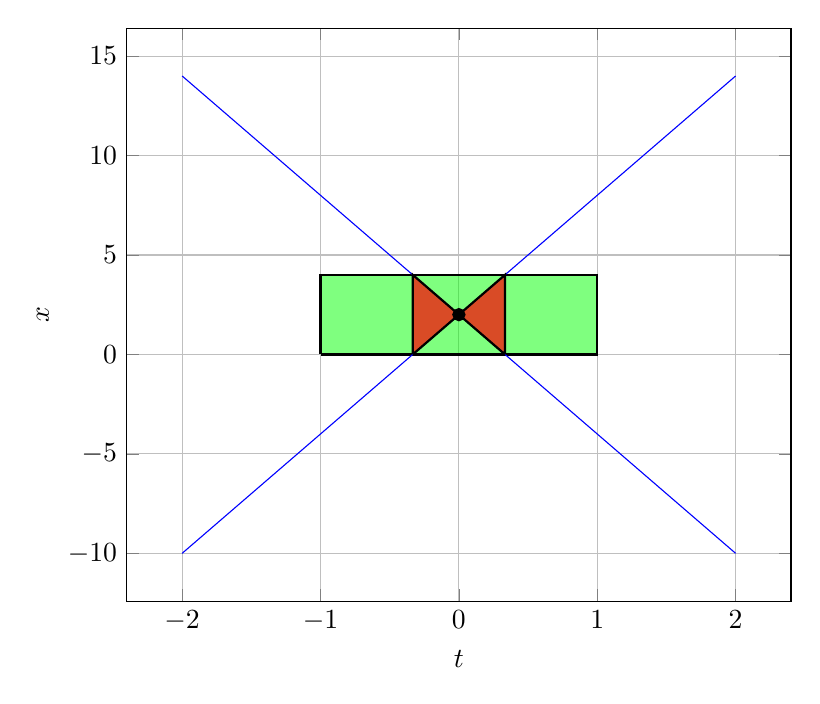
\begin{tikzpicture}
    \begin{axis} [
        scale only axis,
        grid=major,
        xlabel = $t$,
        ylabel = $x$,
      ]
      %\addplot[color=black,thick,fill=gray, fill opacity=0.5, smooth] coordinates {(-2,-3)(0,-4)(3,-2)(2,6)(0,10)(-2.5,6)(-3,0)(-2,-3)};
      \addplot[color=black,thick,fill=green, fill opacity=0.5] coordinates {(-1,0)(1,0)(1,4)(-1,4)(-1,0)};
      \addplot[color=black,thick,mark=*] coordinates {(0,2)};
      \addplot[color=blue,domain=-2:2]{-6*x+2};
      \addplot[color=blue,domain=-2:2]{6*x+2};
      \addplot[color=black,thick,fill=red, fill opacity=0.7] coordinates {(1/3,0)(1/3,4)(0,2)(1/3,0)};
      \addplot[color=black,thick,fill=red, fill opacity=0.7] coordinates {(-1/3,0)(-1/3,4)(0,2)(-1/3,0)};
      %\node at (axis cs:3,-4) {$\mathcal{D}$};
      %\node at (axis cs: 
    \end{axis}
  \end{tikzpicture}
\end{figure}

\end{enumerate}

\end{proof}

\section{2/12/16: Separable and First-Order Linear Equations}

\subsection{Multiplicatively Separable Functions}
\[ F(t,x) = f(t)g(x) \]
A non-example of a separable function is $F(t,x) = t^2 + x^2$. An example is $F(t,x) = t^2x^3$. \\ \\ 
For our purposes, we will work with first-order ODE's with scalar functions.

\subsection{Separable ODE}
\[ \boxed{x' = f(t)g(x)} \]

There are other ways we can write this equation:
\begin{itemize}
\item \textbf{General Form}: $G(t,x,x') = 0$
\item \textbf{Standard Form}: $\phi(t)x' = F(t,x)$
\begin{itemize}
\item \textbf{Regular Case}: $x' = F(t,x)$, $F$ is the ``slope function''
\item \textbf{Singular Case}: This is when we solve in an interval $(t_0 - \delta, t_0 + \delta)$ where $\delta > 0$ and $\phi(t_0) = 0$.
\end{itemize}
\end{itemize}

To solve this type of equation:
\[
\begin{aligned}
x'(t) &\equiv f(t)g(x(t)) \\
\frac{x'(t)}{g(x(t))} &= f(t) \\
\int_a^t \frac{x'(\tau)}{g(x(\tau))} \ d\tau &= \int_a^t f(\tau) \ d\tau \\
\end{aligned}
\]
Letting $u = x(\tau)$ and $du = x'(\tau) \ d\tau$:

\[
\begin{aligned}
\underbrace{\int_{x(a)}^{x(t)}\frac{du}{g(u)}}_{G(x(t))} &= \underbrace{\int_a^t f(\tau) \ d\tau}_{F(t)} \\
\Aboxed{G(x(t)) &= F(t)}
\end{aligned}
\]

\subsection{Example}
\[ 
\begin{aligned}
x' &= t^2x^3 \\
\frac{x'}{x^3} &= t^2 \\
\int \frac{dx}{x^3} &= \int t^2 \ dt + C \\
\frac{x^{-2}}{-2} &= \frac{t^3}{3} + C \\
x^{-2} &= C - \frac{2}{3}t^3 \\
x &= \pm \dfrac{1}{\sqrt{C - \frac{2}{3}t^3}}
\end{aligned}
\]

\section{2/22/16: Separable Equations, First-Order Linear Equations; Uniqueness for $C^1$ IVP's}

Recall our form for the separable equation:
\[ x' = f(t)g(x) \]
Assume $f$ and $g$ are continuous on their respective domains, $f$ on $I = (t_0 - a,t_0 + a), a>0$, $g$ on $J = (x_0 - b,x_0 + b), b>0$. Let $\mathcal{R} = I \times J$. If we also have $x(t_0) = x_0$, then we have an IVP (initial value problem) on our hands.

But the problem is, $\frac{1}{g(x)}$ isn't necessarily continuous. \\ \\

Separately, solve the algebraic equation $g(x) = 0$ in the interval $J$. Assume for simplicity that the roots of $g$ are isolated and $C^{\infty}$ (``smooth''). Then, we can partition $J$ into open subintervals $J_1,J_2,\dots,J_n$, i.e. \[J = \{a,b,c,d\}\cup J_1\cup J_2\cup \dots \cup J_n\]

\section{2/23/16: Uniqueness for $C^1$ IVP's}
\[ x' = f(t)g(x) \qquad x = x(t) \]
\[ x' \equiv f(t)g(x(t)) \text{ for all } t \in I \]
Assume: $f,g$ have continuous derivatives on their respective domains. Then, all solutions are given as follows: Suppose $g(x)$ has domain $J$. If $a$ and $b$ are consecutive isolated roots of $g$, we can solve on $(a,b)$ as we did yesterday: \[ \underbrace{\int_c^{x(t)}\frac{1}{g(u)} \ du}_{G_c(x(t))} = \underbrace{\int_{t_0}^t f(\tau) \ d\tau}_{F(t)} \qquad \text{where } c \in (a,b) \text{ is arbitrary} \]
\begin{tikzpicture}[scale=0.9]
  \begin{axis}[
      axis lines=middle,clip=false,ticks=none,
      xlabel=$x$,ylabel=$y$,
      xmin=-3,ymin=-3,xmax=10,ymax=10,
    ]
    \addplot[smooth] coordinates {(0.5,9)(1,5)(2,2)(3,-2)(4,-1)(4.5,3)};
  \end{axis}
\end{tikzpicture}  % FIX THIS LATER

If $a$ is a root of $g$ (isolated or not) then claim: $x(t) \equiv a$ for $t \in \mathbb{R}$ is a solution of the differential equation.

\subsection{Uniqueness} 
Are these all the solutions, however? \\ \\
A first-order IVP in standard form (the regular case): \[ x' = \underbrace{F(t,x)}_{\text{slope function}}, \qquad x(t_0) = x_0 \]
\underline{Assumption}: $F$ is a $C^1$ function ($\frac{\partial F}{\partial t}$ and $\frac{\partial F}{\partial x}$ are both continuous) on a rectangle centered at the initial point $(t_0,x_0)$. Then, we have the following theorem:
\begin{theorem}
If $\phi(t)$ and $\psi(t)$ are solutions of the IVP, defined on respective domains $I_{\delta} = (t_0 - \delta,t_0 + \delta)$ and $I_{\varepsilon} = (t_0 - \varepsilon,t_0 + \varepsilon)$ where $\delta > 0$ and $\varepsilon > 0$, then \[ \phi(t) \equiv \psi(t) \] for all $t \in I_{\eta} = (t_0 - \eta, t_0 + \eta)$ where $\eta > 0$.
\end{theorem}
Basic outline for the proof: \[ \text{IVP} \qquad x'(t) \equiv F(t,x(t)), \qquad x(t_0) = x_0 \]
\[ x(t) - x(t_0) = \int_{t_0}^t F(\tau,x(\tau)) \ d\tau \]

\section{2/24/16: Uniqueness \& Existence for $C^1$ IVP's}
\subsection{Autonomous Equations and the Time Shift Property}
\[
\begin{cases}
x' = \sqrt{|x|} \qquad \text{(autonomous -- the independent variable makes no explicit appearance)} \\
x(0) = 0
\end{cases}
\]

One important property of an autonomous differential equation is that it is time-indepedent, i.e. if $x = \phi(t)$ is a solution, then so is $x = \psi(t) \coloneqq \phi(t+c)$. Without an initial condition, we have an infinite number of solutions. 

Let us try separation of variables:
\[ 
\begin{aligned}
\int_0^{x(t)} \frac{dx}{\sqrt{|x|}} &= \int_0^t d\tau = t \\
\lim_{\varepsilon \to 0^+}\int_{\varepsilon}^{x(t)} u^{-\frac{1}{2}} \ du &= \lim_{\varepsilon \to 0^+}\left[2u^{\frac{1}{2}}\right]_{\varepsilon}^{x(t)} \\
&= 2\sqrt{x(t)} - \lim_{\varepsilon \to 0^+}{\sqrt{\varepsilon}} \\
&= 2\sqrt{x(t)} \\
x(t) &= \frac{t^2}{4} > 0 \quad \text{(assuming $t \ge 0)$}
\end{aligned}
\]
We can similarly derive, for $t \le 0$, that $x(t) = -\frac{t^2}{4}$. We can then construct our function:
\[ x(t) = 
\begin{cases}
\frac{t^2}{4}, \quad t \ge 0 \\
-\frac{t^2}{4}, \quad t < 0
\end{cases}
\]
\subsection{Unique Solutions}
\begin{center}
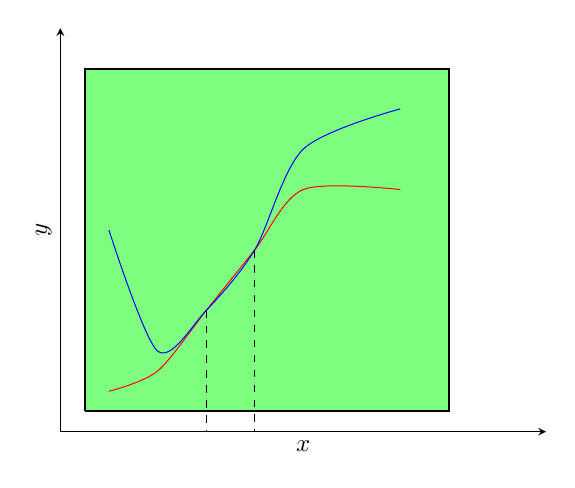
\begin{tikzpicture}[scale=0.9]
  \begin{axis}[
      axis lines=left,clip=false,ticks=none,
      xlabel=$x$,ylabel=$y$,
      xmin=0,ymin=0,xmax=10,ymax=10,
    ]
    \addplot[color=black,thick,fill=green, fill opacity=0.5] coordinates{(0.5,0.5)(8,0.5)(8,9)(0.5,9)(0.5,0.5)};
    \addplot[color=red,smooth] coordinates {(1,1)(2,1.5)(3,3)(4,4.5)(5,6)(7,6)};
    \addplot[color=blue,smooth] coordinates {(1,5)(2,2)(3,3)(4,4.5)(5,7)(7,8)};
    \draw[dashed] (axis cs:3,3) -- (axis cs:3,0);
    \draw[dashed] (axis cs:4,4.5) -- (axis cs:4,0);
    %\node[below] at (axis cs:3,0) {
  \end{axis}
\end{tikzpicture}
\end{center}
\begin{proof}
We begin by showing that our IVP is actually an integral equation.
\[
\boxed{
\begin{cases}
x'(t) \equiv F(t,x(t)) \\
x(t_0) = x_0
\end{cases}}
\]
\[
\begin{aligned}
x'(\tau) &\equiv F(\tau,x(\tau)) \\
\int_{t_0}^tx'(\tau) \ d\tau &= \int_{t_0}^t F(\tau,x(\tau)) \ d\tau \\
\Aboxed{x(t) &= x_0 + \int_{t_0}^tF(\tau,x(\tau)) \ d\tau, \quad \text{$x(t)$ is continuous}}
\end{aligned}
\]
We have just proved one direction of equivalence. To prove the other direction, note that $x(t)$ is differentiable, since all of its parts are continuous and differentiable.
\end{proof}

\section{2/25/16: Uniqueness/Existence for $C^1$ IVP's}
We're assuming: for $\delta > 0$, $\varepsilon > 0$:
\[ \phi: I_{\delta} \coloneqq (t_0 - \delta, t_0 + \delta) \to \mathbb{R} \text{ satisfies } \phi'(t) \equiv F(t,\phi(t)), \phi(t_0) = x_0 \]
\[ \psi: I_{\varepsilon} \coloneqq (t_0 - \varepsilon, t_0 + \varepsilon) \to \mathbb{R} \text{ satisfies } \psi'(t) \equiv F(t,\psi(t)), \psi(t_0) = x_0 \]
We want to show that for some $\eta > 0$, $\phi(t) \equiv \psi(t)$ on $I_{\eta} \coloneqq (t_0 - \eta,t_0 + \eta)$. 

First, we introduce the following concept:
\begin{definition}
If $f$ is a bounded real-valued function on a set $\mathcal{S}$, then its \textbf{sup-norm} is defined as: 
\[ \|f\|_{\mathcal{S}} \coloneqq \sup_{x \in \mathcal{S}}|f(x)| \]
If $\mathcal{S}$ is a closed, bounded subset of $\mathbb{R}^n$, and $f$ is continuous, then $\norm{f}_{\mathcal{S}} = \displaystyle\max_{x \in \mathcal{S}}|f(x)|$ , in which case is called the \textbf{max-norm}.
\end{definition}

Note that:
\begin{itemize}
\item $\norm{f}_{\mathcal{S}} \ge 0$
\item $\norm{f}_{\mathcal{S}} = 0$ iff $f(x) \equiv 0$ for all $x \in \mathcal{S}$
\item $\norm{\alpha f}_{\mathcal{S}} = |\alpha|\norm{f}_{\mathcal{S}}$
\item $\norm{f + g}_{\mathcal{S}} \le \norm{f}_{\mathcal{S}} + \norm{g}_{\mathcal{S}}$ where $f$ and $g$ are defined and bounded on $\mathcal{S}$.
\end{itemize}

We claim that $\norm{\phi - \psi}_{I_{\eta}} \le c \norm{\phi - \psi}_{I_{\eta}}$, where $0 < c < 1$. This would mean that $\norm{\phi - \psi}_{I_{\eta}} = 0$, then $\phi(t) - \psi(t) \equiv 0$ on $I_{\eta}$ and $\phi(t) = \psi(t)$ on $I_{\eta}$.

\begin{proof}
Note that \[ \phi(t) \equiv x_0 + \int_{t_0}^tF(\tau, \phi(\tau)) \ d\tau \] for all $t \in I_{\delta}$ and \[ \psi(t) \equiv x_0 + \int_{t_0}^t F(\tau,\psi(\tau)) \ d\tau \] for all $t \in I_{\varepsilon}$. Both of these equation are true for all $t \in I_{\min(\delta,\varepsilon)}$.

Restrict $t \in I_{\eta}$ where $0 \le \eta \le \min(\delta,\varepsilon)$. Subtracting these two equations:
\[ 
\begin{aligned}
|\phi(t) - \psi(t)| &= \left| \int_{t_0}^t[F(\tau,\phi(\tau)) - F(\tau,\psi(\tau))] \ d\tau \right| \\
&\le \left| \int_{t_0}^t|F(\tau,\phi(\tau)) - F(\tau,\psi(\tau))| \ d\tau\right| \\
\text{(MVT)} \qquad &\le \left| \int_{t_0}^t\underbrace{\left|\frac{\partial F}{\partial x}(x,\theta(\tau))\right|}_{\le M}\left|\phi(t) - \psi(t)\right| \ d\tau \right| \\
&\le M\left|\int_{t_0}^t\underbrace{|\phi(\tau) - \psi(\tau)|}_{\le \norm{\phi - \psi}_{I_{\eta}}} \ d\tau \right| \\
&\le M\norm{\phi - \psi}(t-t_0) \le M\eta\norm{\phi - \psi}_{I_{\eta}}
\end{aligned}
\]

Now we simply pick $\eta$ such that $M\eta = c < 1$, and we are done. 
\end{proof}

\section{2/26/16: Existence}
\subsection{Transforming to an Integral Equation}
Yesterday we proved the uniqueness of the solution of an IVP. Now we must prove the existence. 

\[
\begin{cases}
x' = F(t,x), \qquad x = x(t) \text{ is the unknown function} \\
x(t_0) = x_0
\end{cases}
\]
$C^1$ IVP $\Leftrightarrow$ $F(t,x)$ is $C^1$ in some rectangle $\mathcal{R}$ centered at $(x_0,y_0)$.

Let us integrate our equation:
\[ 
\begin{aligned}
\int_{t_0}^t x'(\tau) \ d\tau &= \int_{t_0}^t F(\tau,x(\tau)) \ d\tau \\
x(t) - x(t_0) = x(t) - x_0 &= \int_{t_0}^t F(\tau,x(\tau)) \ d\tau \\
\end{aligned}
\]

So now our problem/equation becomes:
\begin{itemize}
\item $x(t) \equiv x_0 + \displaystyle\int_{t_0}^t F(\tau,x(\tau)) d\tau$
\item $x(t)$ is a continuous function of $t$
\end{itemize}
Why do we need the continuity condition? If $x(t)$ is a solution, then it is differentiable, which implies it is continuous. 

Now we prove the opposite direction. To prove that $x(t)$ is differentiable, note that $f(t) = x_0$ is differentiable, and the integral is also differentiable (since its derivative is $F(t,x(t))$, which is continuous. Therefore, by algebra, the two statements are equivalent.

\subsection{Picard's Method}

Define \[ x_{n+1}(t) \coloneqq x_0 + \int_{t_0}^t F(\tau, x_n(\tau)) \ d\tau \]
and
\[ x_0(t) :\equiv x_0 \quad \text{for all } t \]

In this section, we prove that for each $t \in I_{\eta}$, $\displaystyle\lim_{n \to \infty}x_n(t)$ exists, let's call it $x(t)$, and moreover: 
\begin{itemize}
\item $x(t)$ is a continuous function of $t$ on $I_{\eta}$
\item $x(t) \equiv x_0 + \displaystyle\int_{t_0}^t F(\tau, x(\tau)) \ d\tau$
\end{itemize}

\begin{center}
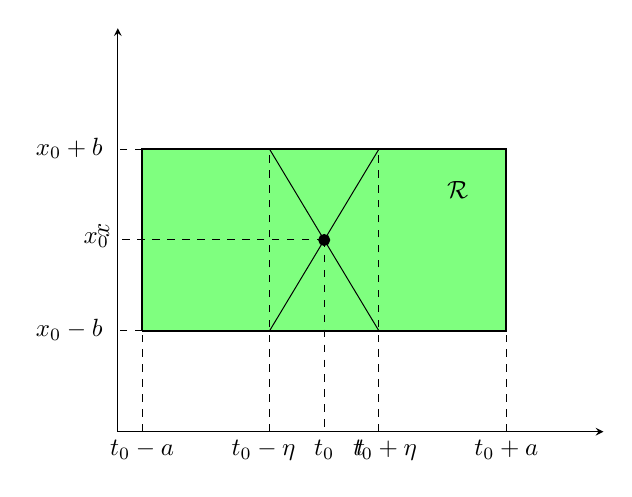
\begin{tikzpicture}[scale=0.9]
  \begin{axis}[
      axis lines=left,clip=false,ticks=none,
      xlabel=$t$,ylabel=$x$,
      xmin=0,ymin=0,xmax=10,ymax=10,
    ]
    \addplot[color=black,thick,fill=green, fill opacity=0.5] coordinates{(0.5,2.5)(8,2.5)(8,7)(0.5,7)(0.5,2.5)};
    \addplot[color=black,thick,mark=*] coordinates {(4.25,4.75)};
    \draw[dashed] (axis cs: 4.25,4.75) -- (axis cs: 4.25,0);
    \draw[dashed] (axis cs: 4.25,4.75) -- (axis cs: 0,4.75);
    \node[below] at (axis cs:4.25,0) {$t_0$};
    \node[left] at (axis cs: 0,4.75) {$x_0$};
    \addplot[color=black,domain=3.125:5.375]{2*x-3.75};% draw lines of slopes M and -M through the point
    \addplot[color=black,domain=3.125:5.375]{-2*x+13.25};
    \draw[dashed] (axis cs: 5.375,0) -- (axis cs: 5.375,7);
    \draw[dashed] (axis cs: 3.125,0) -- (axis cs: 3.125,7);
    \draw[dashed] (axis cs: 0.5,0) -- (axis cs: 0.5,2.5);
    \draw[dashed] (axis cs: 8,0) -- (axis cs: 8,2.5);
    \draw[dashed] (axis cs: 0.5,2.5) -- (axis cs: 0,2.5);
    \draw[dashed] (axis cs: 0.5,7) -- (axis cs: 0,7);
    \node[below] at (axis cs: 3,0) {$t_0 - \eta$};
    \node[below] at (axis cs: 5.5,0) {$t_0 + \eta$};
    \node[below] at (axis cs: 0.5,0) {$t_0 - a$};
    \node[below] at (axis cs: 8,0) {$t_0 + a$};
    \node[below] at (axis cs: -1,3) {$x_0 - b$};
    \node[below] at (axis cs: -1,7.5) {$x_0 + b$};
    \node at (axis cs: 7,6) {$\mathcal{R}$};
  \end{axis}
\end{tikzpicture}
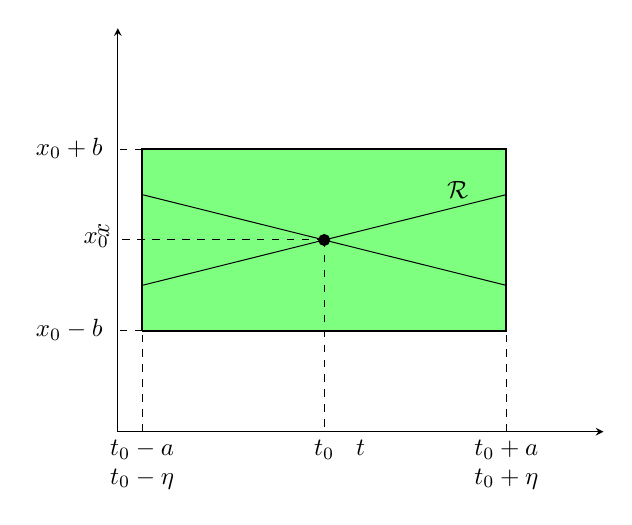
\begin{tikzpicture}[scale=0.9]
  \begin{axis}[
      axis lines=left,clip=false,ticks=none,
      xlabel=$t$,ylabel=$x$,
      xmin=0,ymin=0,xmax=10,ymax=10,
    ]
    \addplot[color=black,thick,fill=green, fill opacity=0.5] coordinates{(0.5,2.5)(8,2.5)(8,7)(0.5,7)(0.5,2.5)};
    \addplot[color=black,thick,mark=*] coordinates {(4.25,4.75)};
    \draw[dashed] (axis cs: 4.25,4.75) -- (axis cs: 4.25,0);
    \draw[dashed] (axis cs: 4.25,4.75) -- (axis cs: 0,4.75);
    \node[below] at (axis cs:4.25,0) {$t_0$};
    \node[left] at (axis cs: 0,4.75) {$x_0$};
    \addplot[color=black,domain=0.5:8]{0.3*x+3.475};% draw lines of slopes M and -M through the point
    \addplot[color=black,domain=0.5:8]{-0.3*x+6.025};
    \draw[dashed] (axis cs: 0.5,0) -- (axis cs: 0.5,2.5);
    \draw[dashed] (axis cs: 8,0) -- (axis cs: 8,2.5);
    %\draw[dashed] (axis cs: 0.5,5.875) -- (axis cs: 0,5.875);
    %\draw[dashed] (axis cs: 0.5,3.625) -- (axis cs: 0,3.625);

    \draw[dashed] (axis cs: 0.5,2.5) -- (axis cs: 0,2.5);
    \draw[dashed] (axis cs: 0.5,7) -- (axis cs: 0,7);
    \node[below] at (axis cs: 0.5,-0.7) {$t_0 - \eta$};
    \node[below] at (axis cs: 8,-0.7) {$t_0 + \eta$};
    \node[below] at (axis cs: 0.5,0) {$t_0 - a$};
    \node[below] at (axis cs: 8,0) {$t_0 + a$}; % FIX THIS FAST PLEASE YEAH
    \node[below] at (axis cs: -1,3) {$x_0 - b$};
    \node[below] at (axis cs: -1,7.5) {$x_0 + b$};
    \node at (axis cs: 7,6) {$\mathcal{R}$};
  \end{axis}
\end{tikzpicture}
\end{center}
Define $M \ge \displaystyle\max_{(t,x) \in \mathcal{R}}|F(t,x)|$ (existence follows from EVT). Let $\eta \coloneqq \min(a,\frac{b}{M}) > 0$. Assume $M>0$; if $M=0$, then the IVP is $x' \equiv 0$, $x(t_0) = x_0$ has a solution: $x(t) \equiv x_0$ for all $t \in (t_0 - a,t_0 + a)$.

\section{2/29/16: Picard's Existence Proof, Continued...}
Recapping: our base function is \[ x_0(t) \equiv x_0 \qquad \text{for all } t \in I_{\eta}, \eta = \min\left(a,\frac{b}{M}\right) >0 \]

We need to choose the size of the rectangle for each function. In the example 
\[
\begin{cases}
x' = t^2 + x^2 \\
x(0) = 1
\end{cases}
\]

We need to find some $\eta > 0$ such that a solution is guaranteed to exist in $(-\eta,\eta)$. Let $\mathcal{R} = [-T,T] \times [1-r,1+r]$ be our rectangle. Then take $M = T^2 + (1+r)^2$, then $|t^2 + x^2| \le M$ when $(t,x) \in \mathcal{R}$.

\subsection{Proving Well-Defined-ness}
\begin{theorem}
Each $x_n$ is well-defined and continuous and satisfies $|x_n(t) - x_0| \le b$ for all $t \in I_{\eta}$.
\end{theorem}
\begin{proof}
The base case is trivial. Now assume true for $x_n(t)$; we now prove for $x_{n+1}(t)$. By assumption, the integrand $F(\tau,x_n(\tau))$ is well-defined and continuous (and therefore Riemann integrable on $I_{\eta}$) for all $t \in I_{\eta}$, which means the integral is well-defined. Therefore, $x_{n+1}(t)$ is well-defined for all $t \in I_{\eta}$.

Also, $x_{n+1}(t)$ is continuous on $I_{\eta}$ by similar reasoning. 

Now, we investigate $|x_{n+1}(t) - x_0$. First, we claim that $(\tau, x_n(\tau)) \in \mathcal{R}$ for any $\tau$ between $t_0$ and $t$. But \[ |\tau - t_0| \le |t-t_0| \le \eta \le a\]
\[ |x_n(\tau) - x_0| \le b \]

\[
\begin{aligned}
|x_{n+1}(t) - x_0| &= \left|\int_{t_0}^tF(\tau,x_n(\tau)) \ d\tau \right| \\
&\le \left|\int_{t_0}^t\underbrace{|F(\tau,x_n(\tau))|}_{\le M} \ d\tau \right| \\
&\le M|t-t_0| \le M\eta \le b
\end{aligned}
\]

\end{proof}

\section{3/1/16: Finish Picard's Existence Proof}

\begin{theorem}
\[ |x_{n+1}(t) - x_n(t)| \le \frac{MK^{n}}{(n+1)!}|t-t_0|^{n+1} \]
for any $n \ge 0$ and any $t \in I_{\eta}$, where $K \ge \displaystyle\max_{(t,x) \in \mathcal{R}}\left|\frac{\partial F}{\partial x}(t,x)\right|$ (using the assumed $C^1$-ness of $F$ on $\mathcal{R}$).
\end{theorem}

\begin{proof}
We prove by induction. When $n=0$:
\[ |x_1(t) - x_0(t)| = |x_1(t) - x_0| = \left|\int_{t_0}^tF(\tau,x_0) \ d\tau\right| \le M|t-t_0| = \frac{MK^0}{(0+1)!}|t-t_0|^{0+1} \]
Now assume the hypothesis, we want to prove that \[ |x_{n+2}(t) - x_{n+1}(t)| \le \frac{MK^{n+1}}{(n+2)!}|t-t_0|^{n+2} \]
So:
\[
\begin{aligned}
|x_{n+2}(t) - x_{n+1}(t)| &= \left|\int_{t_0}^tF(\tau,x_{n+1}) - F(\tau,x_n) \ d\tau \right| \\
\text{(MVT, for some } y_n \in [x_n,x_{n+1}]) \qquad &= \left|\int_{t_0}^t\frac{\partial F}{\partial x}(\tau,y_n)(x_{n+1} - x_n) \ d\tau \right| \\
&\le \left|\int_{t_0}^t\left|\frac{\partial F}{\partial x}(\tau,y_n)\right||(x_{n+1} - x_n)| \ d\tau \right|\\
&\le K\left|\int_{t_0}^t|x_{n+1} - x_n|\ d\tau \right| \\
&\le K\left|\int_{t_0}^t\frac{MK^{n}}{(n+1)!}|t-t_0|^{n+1} \ d\tau\right| \\
&= \frac{MK^{n+1}}{(n+2)!}|t-t_0|^{n+2} 
\end{aligned}
\]
\end{proof}

\section{3/3/16}

For any $t \in I_{\eta}$, \[ |x_{n+p}(t) - x_n(t)| = |x_{n+p}(t) - x_{n+p-1}(t) + x_{n+p-1}(t) - x_{n+p-2}(t) + x_{n+p-2}(t) - \cdots - x_n(t) \] is bounded. By the Triangle Inequality,
\[
\begin{aligned}
|x_{n+p}(t) - x_n(t)| &\le \sum_{j=n}^{n+p-1}|x_{j+1}(t) - x_j(t)| \\
&\le \sum_{j=n}^{n+p-1} \frac{MK^j}{(j+1)!}|t-t_0|^{j+1} \\
&= \left(\frac{M}{K}\right) \sum_{j=n}^{n+p-1}\frac{(K|t-t_0|)^{j+1}}{(j+1)!} \\
&\le \left(\frac{M}{K}\right) \sum_{j=n}^{\infty}\frac{(K|t-t_0|)^{j+1}}{(j+1)!}\\
&\le \left(\frac{M}{K}\right) \sum_{j=n}^{\infty}\frac{(K\eta)^{j+1}}{(j+1)!}\\
&= \left(\frac{M}{K}\right)\left(e^{k\eta} - \sum_{j=0}^{n-1}\frac{(k\eta)^{j+1}}{(j+1)!} \right)
\end{aligned}
\]

Thus, we have an upper bound for any two terms in our sequence.

Now if we take $\norm{x_{n+p} - x_n}_{I_{\eta}} = \displaystyle\sup_{t\in I_{\eta}}|x_{n+p}(t) - x_n(t)| \le L$, then send $n \to \infty$. Then, \[ \lim_{n \to \infty}\norm{x_{n+p(n)} - x_n}_{I_{\eta}} \le 0 \]
But this is also nonnegative, so it must be the case that the limit is zero, and thus this sequence is Cauchy.

\section{3/4/16: Existence of Solutions, Continued}
The last thing we proved was that $(x_n)$ is a \underline{Cauchy sequence} in the space of continuous functions on $I_{\eta}$, denoted $C^0(I_{\eta})$, under the sup-norm, $\norm{f}_{I_{\eta}} = \displaystyle\sup_{t \in I_{\eta}}|f(t)|$. This means: $\displaystyle\lim_{n \to \infty} \norm{x_{n+p(n)} - x_n}_{I_{\eta}} = 0$ for any $\mathbb{N}$-valued function $p(n)$.

\subsection{Metric Spaces}
\begin{definition}
A \textbf{metric space}, denoted $(\mathscr{X},d)$, $\mathscr{X}\neq \emptyset$, $d$ is a ``distance'' function, must satisfy the following:
\begin{enumerate}
\item $d:(\mathscr{X}\times \mathscr{X}) \to [0,\infty)$
\item $d(x,y) \ge 0$ and $d(x,y) = 0 \Leftrightarrow x=y$
\item $d(x,y) = d(y,x)$
\item $d(x,y) + d(y,z) \ge d(x,z)$
\end{enumerate}
\end{definition}

If we have a metric $d$ on a vector space $\mathcal{V}$, we can also require $d(x,y) + d(y,z) = d(x,z)$ iff $x\text{-}y\text{-}z$ ($y$ is between $x$ and $z$) or $x=y$ or $y=z$. To define betweenness: $\vec{p}\text{-}\vec{q}\text{-}\vec{r}$ iff $\vec{q} = (1-t)\vec{p} + t\vec{r}$. \\ \\
Here, we define a metric on a vector space. Given a vector space $\mathcal{V}$, a \textbf{norm} on $\mathcal{V}$ is a real-valued function $\norm{\cdot}$ such that:
\begin{enumerate}
\item $\norm{\vec{v}} \ge 0$ and $\norm{\vec{v}} = 0 \Leftrightarrow \vec{v} = \vec{0}$ (Positive definiteness)
\item $\norm{c\vec{v}} = |c|\norm{\vec{v}}$ (Absolute homogeneity)
\item $\norm{\vec{v} + \vec{w}} \le \norm{\vec{v}} + \norm{\vec{w}}$ (Triangle inequality)
\end{enumerate}
This way, we can define \[ d(\vec{v},\vec{w}) \coloneqq \norm{\vec{v} - \vec{w}} \]

\subsection{Cauchy Sequences in Metric Spaces}
In a metric space $(\mathscr{X},d)$, a sequence of elements $(x_n)$ converges to $x \in \mathscr{X}$ if $d(x_n,x) \to 0$ as $n \to \infty$. \\

A sequence $(x_n)$ in $(\mathscr{X},d)$ is called \underline{Cauchy} if $d(x_n,x_m) \to 0$ as $\min(n,m) \to \infty$.

Not all Cauchy sequences converge. As an example, take \[ \mathscr{X} = \mathbb{Q}, \qquad d(q,\tilde{q}) = |q- \tilde{q}| \]
Take the sequence $(3,3.1,3.14,3.141,\cdots)$. This sequence is Cauchy since choosing two far-out values will differ very little. However, it converges to $\pi$, which is not in the metric space. Therefore, we call this an \textbf{incomplete metric space}.


\section{3/7/16: Cauchy Sequences and Convergence in $\mathbb{R}$ and in $C^0([a,b])$}

A sequence $(t_n)$ in $\mathbb{R}$ is \underline{Cauchy} if $|t_n - t_m| \to 0$ as $\min(n,m) \to \infty$. More precisely, $\forall \varepsilon > 0, \exists N: n,m \ge N \Rightarrow |t_n - t_m| < \varepsilon$.

We'd like to prove that every Cauchy sequence in $\mathbb{R}$ converges to some $t \in \mathbb{R}$.

\begin{theorem}
$(\mathbb{R}, |\cdot - \cdot |)$ is a \textbf{complete metric space}, i.e. every Cauchy sequence of real numbers converges to a real limit.
\end{theorem}

We make use of several lemmas. First, a definition:
\begin{definition}
A \textbf{subsequence} of $(t_n)$ is any sequence of the form $(t_{k_n})$ where $(k_n)$ is a strictly increasing sequence of natural numbers: $1 \le k_1 < k_2 < \cdots < k_n < \cdots$
\end{definition}
\begin{definition}
A sequence $(u_n)$ is called \underline{monotone} if either $u_1 \le u_2 \le u_3 \le \cdots \le u_n \le \cdots$ or $u_1 \ge u_2 \ge u_3 \ge \cdots \ge u_n \ge \cdots$.
\end{definition}
\begin{lemma}
A subsequence of a subsequence of $(t_n)$ is itself a subsequence of $(t_n)$.
\end{lemma}
\begin{lemma}
If $(k_n)$ is a strictly increasing sequence in $\mathbb{N}$, then $k_n \to \infty$ as $n \to \infty$. In fact, $k_n \ge n$.
\end{lemma}
\begin{lemma}
Every sequence in $\mathbb{R}$ has a monotone subsequence.
\end{lemma}

\begin{center}
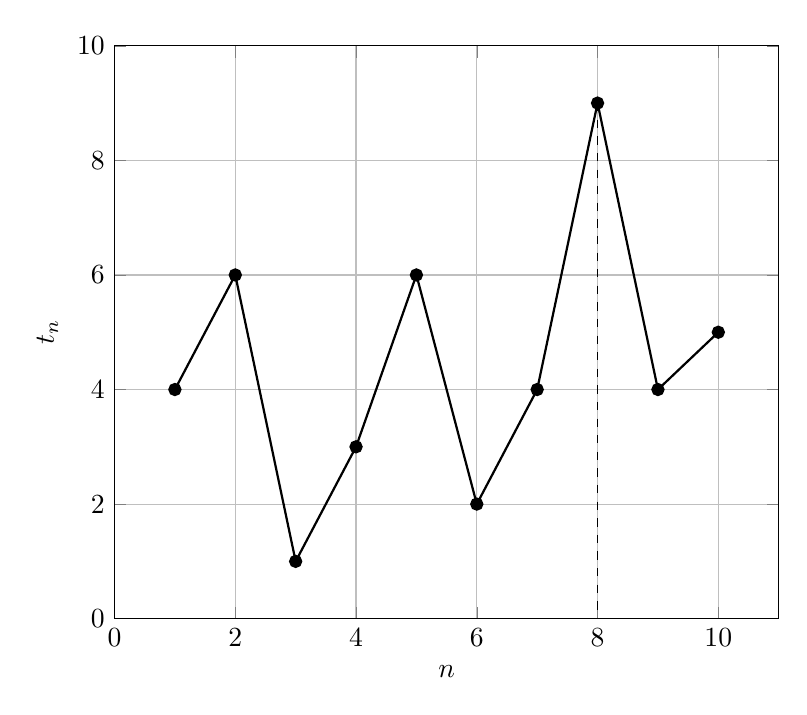
\begin{tikzpicture}
  \begin{axis} [
      scale only axis,
      grid=major,
      inner axis line style={->},
      xmin=0,
      ymin=0,
      xmax=11,
      ymax=10,
      xlabel = $n$,
      ylabel = $t_n$,
    ]
    \addplot[color=black, thick, mark = *] coordinates {(1,4)(2,6)(3,1)(4,3)(5,6)(6,2)(7,4)(8,9)(9,4)(10,5)};
    \draw[dashed] (axis cs:8,9) -- (axis cs:8,0);
    \node[below] at (axis cs:8,0) {$N$};
  \end{axis}
\end{tikzpicture}
\end{center}
\begin{proof}
We call $N$ a \underline{vista} if $t_N > t_{N+k}$ for all $k \ge 1$. We consider two cases:
\begin{enumerate}
\item the set of vistas is infinite; call them $N_1 < N_2 < N_3 < \cdots$. Then, \[ t_{N_1} > t_{N_2} > t_{N_3} > \cdots \] and we can take $(t_{N_n})$ as our subsequence--this is strictly decreasing, so certainly monotone down.
\item the set of vistas is finite (including possibly empty). Then, let $N$ be one more than the greatest among the vistas. $N$ is not a vista, so $\exists k_2 > k_1 = N: t_{k_2} \ge t_{k_1}$. $k_2$ is also not a vista, so $\exists k_3 > k_2: t_{k_3} \ge t_{k_2}$. Then taking $(t_{k_n})$, we have our monotone subsequence.
\end{enumerate}
\end{proof}

\begin{lemma}
Every Cauchy sequence in $\mathbb{R}$ (true in any metric space) is bounded: \[ \exists M: |t_n| \le M \] for all $n \ge 1$.
\end{lemma}

\begin{proof}
By definition, we can choose some $N$ such that \[ n,m \ge N \Rightarrow |t_n - t_m| < 1 \] Take $m = N$, then $|t_n - t_N| < 1$, and \[ |t_N| - 1 \le |t_n| \le |t_N| + 1 \qquad \forall n \ge N\]
\[ |t_n| \le \max(|t_1|,|t_2|,|t_3|,\cdots,|t_{N-1}|) \]
\end{proof}

\end{document}
